% Generated by tools/golden_study/plot_qft96_routes.py; do not edit by hand.
\begin{figure}[H]
\centering
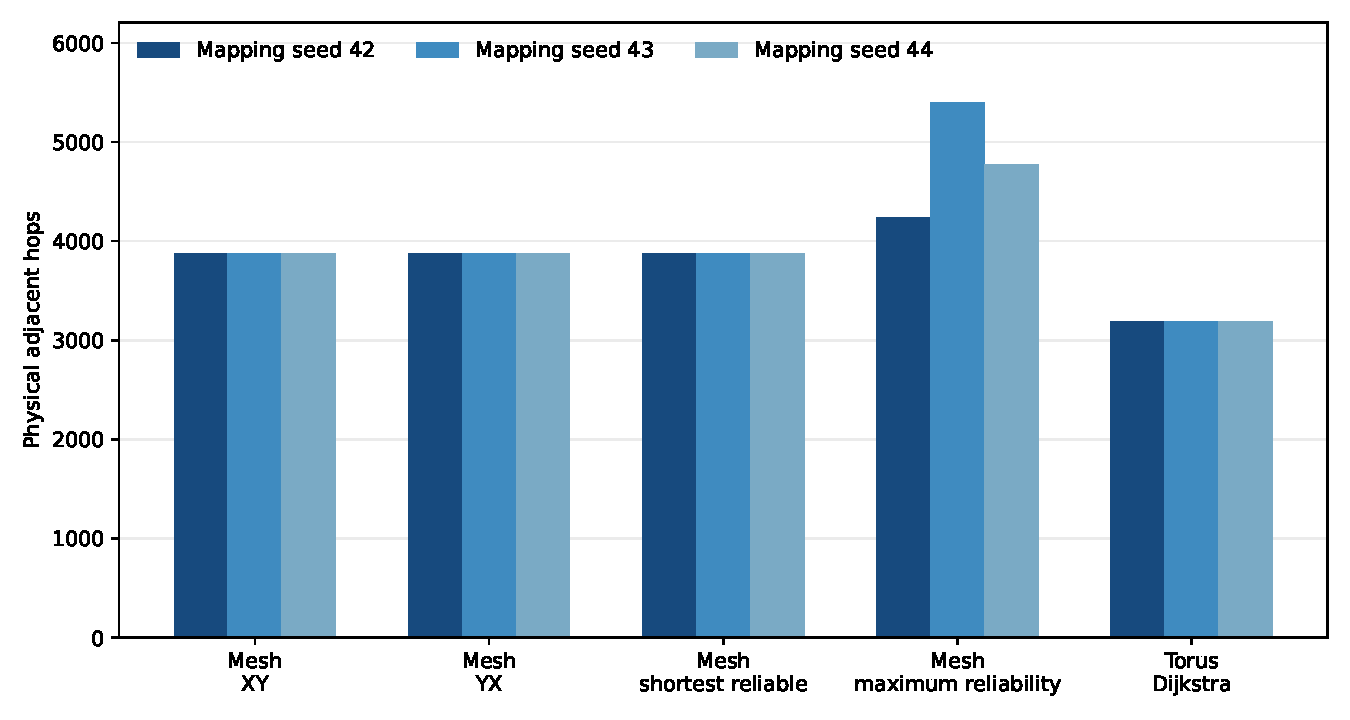
\includegraphics[width=0.78\linewidth]{../../../results/qft96_2seed_2026-10-26/figures/qft96_route_hops.pdf}
\caption{QFT-96 adjacent-hop count on the same T-HQA placement for each seed. Torus uses Dijkstra. These are structural counts, not simulated latency. The complete values are in Table~\ref{tab:qft96-route-hops} and the \href{https://github.com/sanjeevkrishnaa/Compiler-Driven-ACE/blob/codex/ace-scheduler-correctness/results/qft96_2seed_2026-10-26/validation/mapping_audit.csv}{source CSV}.}
\label{fig:qft96-route-hops}
\end{figure}
\begin{table}[H]
\centering\small
\begin{tabular}{lrrr}
\toprule
Route & Seed 42 hops & Seed 43 hops & Seed 44 hops \\
\midrule
Mesh XY & 3876 & 3876 & 3876 \\
Mesh YX & 3876 & 3876 & 3876 \\
Mesh shortest reliable & 3876 & 3876 & 3876 \\
Mesh maximum reliability & 4242 & 5396 & 4774 \\
Torus Dijkstra & 3186 & 3186 & 3186 \\
\bottomrule
\end{tabular}
\caption{Exact QFT-96 route counts for all three mapping seeds. Every row has 1,965 logical migrations and 766 layers. \href{https://github.com/sanjeevkrishnaa/Compiler-Driven-ACE/blob/codex/ace-scheduler-correctness/results/qft96_2seed_2026-10-26/validation/mapping_audit.csv}{Source CSV}.}
\label{tab:qft96-route-hops}
\end{table}
